\documentclass[12pt,a4paper]{article}
\usepackage{tpl}
\usepackage{chessboard}
\dbegin{Кружок для 7 класса, продолжающие, школа №179}{Решения занятия №16}

\z Таблица $9\times10$ заполнена числами $0,1,-1$ так, что сумма чисел в любом квадрате $3\times3$ равна нулю. Какое наибольшее значение может принимать сумма всех чисел таблицы?

\s Разделим таблицу на квадрат $9\times9$ и прямоугольник $9\times1$. Сумма в квадрате 0, значит, сумма в таблице не больше 9. Пример на 9 изображён ниже.\QEDA\\

\n В город приехали 60 певцов из двух стран --- Франции и Германии. Каждый день два певца из разных стран дают концерт, при этом пары певцов не должны повторяться. Какое наибольшее количество концертов они смогут дать?

\s Можно считать, что певцов из Германии не больше. Пусть их $30-k$, тогда певцов из Франции $30+k$. Тогда максимальное количество концертов --- $(30-k)(30+k)=900-k^2$. Это число максимально, когда $k=0$ и равно 900.\QEDA

\p То же, но певцов 75.

\s Аналогично предыдущему пункту получаем, что если певцов из Германии $37.5-k$, то концертов $37.5^2-k^2$. При этом $k$ должно быть полуцелым и при этом не целым, то есть $k^2\geq\frac14$. Значит, максимум этого выражения равен $37\cdot38=1406$.\QEDA\\

\z Город представляет из себя квадрат $3\times3$, в котором каждая сторона квартала - участок улицы длины 500 метров. Какой наименьший путь придется проделать катку, чтобы заасфальтировать улицы?\label{katok}

\s Чтобы каток мог пройти весь город, должно быть не более 2 перекрёстков, из каждого из которых выходит нечётное количество дорог. У нас таких перекрёстков 8, значит, нужно соединить их ещё как минимум 3 дорогами, а минимальная длина дороги --- 500 метров. Значит, меньше чем $13.5$ километрами обойтись не получится. Пример на $13.5$ километров изображён ниже.\QEDA\\

\z Том Сойер решил покрасить очень длинный забор так, что любые две доски, между которыми либо ровно две, либо ровно три другие, покрашены в разные цвета. Какое наименьшее количество красок понадобится Тому?

\s Пример на 3 цвета такой: первые 2 доски красные, потом 2 синие доски, потом 2 зелёные, потом ещё 2 красные, ещё 2 синие, 2 зелёные и т.п. Допустим, Тому удалось покрасить забор в 2 цвета. Пронумеруем доски. Пусть доска под номером 1 красная. Тогда доски 4 и 5 синие, доска 2 красная, доска 6 синяя, доска 10 красная, тогда доска 7 не может быть красной (т.к. 10 красная) и не может быть синей (т.к. 4 синяя) --- противоречие.

\z Каждый участник шахматного турнира сыграл с каждым по одному разу. За победу давалось 1 очко, за ничью --- $0.5$ очка, за поражение --- $0$. Оказалось, что среди любых трёх участников найдётся шахматист, набравший с партиями с двумя другими ровно $1.5$ очка. Какое наибольшее количество шахматистов могло участвовать в турнире?

\s Пример на 5 игроков --- когда они выигрывают друг у друга по циклу (1 у 2, 2 у 3 и т.п.) и <<несоседние>> игроки (1 и 3, 2 и 4 и т.п.) играют друг с другом вничью. Заметим, что каждый выиграл максимум у одного, т.к. если кто-то выиграл у двоих, то можно взять этих трёх шахматистов и никто из них не выиграл ровно 1.5 очка. Значит, какой-то шахматист проиграл максимум одному. Если игроков хотя бы 6, то этот шахматист сыграл вничью хотя бы с тремя, т.е. среди этих трёх игроков никакие двое не сыграли вничью --- противоречие.\QEDA\\

\z Какое максимальное количество ферзей, не бьющих друг друга, можно расставить на доске: \p $5\times5$? \p $8\times8$?

\s Примеры на соответственно 5 и 8 ферзей изображены ниже. Оценки на 5 и 8 следуют из того, что всего вертикалей на доске соответственно 5 и 8 и на каждой вертикали не может стоять больше 1 ферзя.\QEDA\\

\newpage
\z За круглым столом сидят рыцари и лжецы, всего 100 человек. На вопрос <<Верно ли, что оба ваших соседа рыцари?>> утвердительно ответило столько же людей, сколько всего среди собравшихся лжецов. При каком наименьшем количестве лжецов такое возможно?

\s Оценка: заметим, что число лжецов, сидящих между двумя рыцарями + число лжецов, не сидящих между двумя рыцарями, равно числу рыцарей, сидящих между двумя рыцарями + числу лжецов, не сидящих между двумя рыцарями. То есть рыцарей между двумя рыцарями столько же, сколько и лжецов между двумя рыцарями. Пусть лжецов $k$. Тогда рыцарей между двумя рыцарями не больше $k$. Также заметим, что групп из сидящих подряд лжецов тоже не больше $k$, а значит, групп из сидящих подряд рыцарей максимум $k$. В каждой группе из сидящих подряд рыцарей не больше двух, сидящих с краю, а остальные сидят посередине, каждый между двумя рыцарями. Тогда рыцарей, сидящих рядом со лжецами максимум $2k$. Всего человек не больше $4k$, с другой стороны, их 100, значит, $k\geq 25$. Пример на 25 лжецов получается так. Разобьём стол на 25 секций по 4 человека и в каждую поставим трёх рыцарей, а затем лжеца. \QEDA

\begin{figure}[!htb]
	\begin{minipage}{0.26\textwidth}\centering
		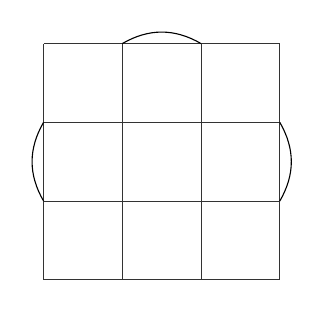
\begin{tikzpicture}
			\draw[step=1,black!80] (0,0) grid (3,3);
			\draw (0,1) to[bend left](0,2);	
			\draw (1,3) to[bend left](2,3);	
			\draw (3,2) to[bend left](3,1);	
		\end{tikzpicture}
		\caption{$13.5$ км в \ref{katok}}
	\end{minipage}
	\begin{minipage}{0.32\textwidth}\centering
		\setchessboard{showmover=false,setpieces={Qa1,Qd2,Qb3,Qe4,Qc5}}
		\chessboard[maxfield=e5]
		\caption{5 ферзей на доске $5\times5$}
	\end{minipage}
	\begin{minipage}{0.38\textwidth}\centering
		\setchessboard{showmover=false,setpieces={Qa3,Qb6,Qc2,Qd7,Qe5,Qf1,Qg8,Qh4}}
		\chessboard
		\caption{8 ферзей на доске $8\times8$}
	\end{minipage}
\end{figure}
\begin{figure}[!htb]
	\begin{minipage}{0.96\textwidth}\centering
		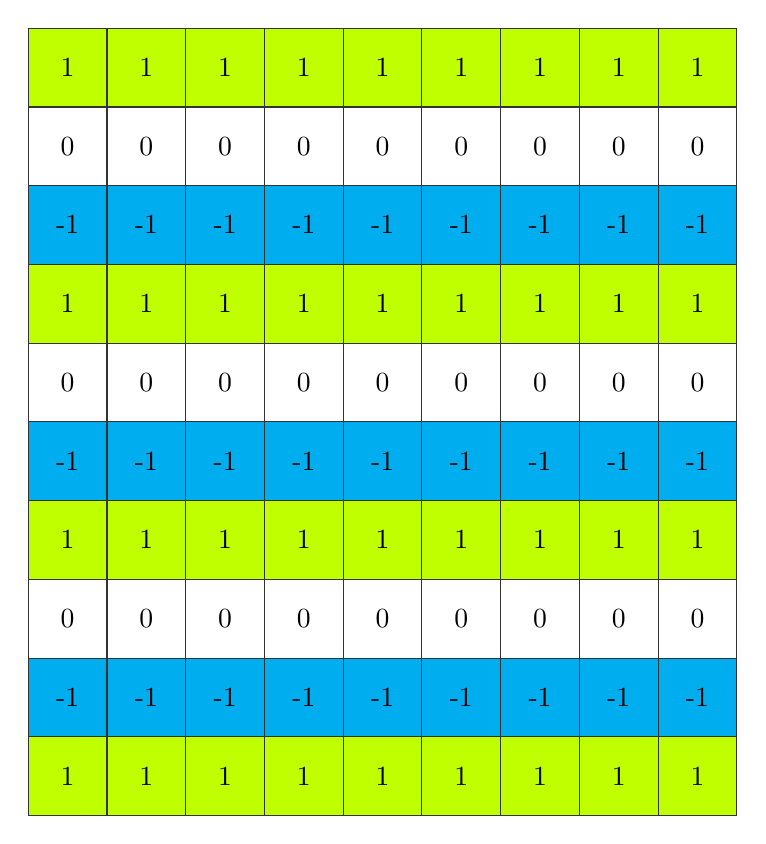
\begin{tikzpicture}
			\draw[fill=lime] (0,0) -- (0,1) -- (9,1) -- (9,0) -- cycle;
			\draw[fill=cyan] (0,1) -- (0,2) -- (9,2) -- (9,1) -- cycle;
			\draw[fill=lime] (0,3) -- (0,4) -- (9,4) -- (9,3) -- cycle;
			\draw[fill=cyan] (0,4) -- (0,5) -- (9,5) -- (9,4) -- cycle;
			\draw[fill=lime] (0,6) -- (0,7) -- (9,7) -- (9,6) -- cycle;
			\draw[fill=cyan] (0,7) -- (0,8) -- (9,8) -- (9,7) -- cycle;
			\draw[fill=lime] (0,9) -- (0,10) -- (9,10) -- (9,9) -- cycle;
			\draw[step=1,black!80] (0,0) grid (9,10);
			\foreach \x in {0.5,3.5,6.5,9.5}
				\foreach \y in {0.5,...,8.5}
					\node at (\y,\x) {1};
			\foreach \x in {1.5,4.5,7.5}
				\foreach \y in {0.5,...,8.5}
					\node at (\y,\x) {-1};
			\foreach \x in {2.5,5.5,8.5}
				\foreach \y in {0.5,...,8.5}
					\node at (\y,\x) {0};
		\end{tikzpicture}
		\caption{Числа на доске $9\times10$}
	\end{minipage}
\end{figure}

\newpage\hdr{Дорешка}

\z Имеется $12$ одинаковых по виду монет, из которых одна фальшивая, отличающаяся по весу от настоящих, и двухчашечные весы без гирь. Как за наименьшее число взвешиваний найти фальшивую монету и узнать, легче она или тяжелее настоящих?

\s Минимальное количество взвешиваний --- $3$.

\textit{Оценка.} Даже если известно, что фальшивая монета легче настоящих, то за $2$ взвешивания можно обработать максимум $9$ монет (частный случай задачи, которая была на одном из предыдущих занятий). Значит, $2$ взвешиваний не хватит.

\textit{Алгоритм.} Первое взвешивание сделаем такое: разделим монеты на три кучи по четыре монеты (пусть это кучи из монет $1-4$, $5-8$, $9-12$) и взвесим первые две кучи. Тогда:

\begin{itemize}
	\item Пусть кучи равны по весу. Тогда у нас остались монеты $9-12$, одна из которых фальшивая, и $8$ заведомо настоящих монет. Взвесим $9,10$ и $11,1$. Если эти кучи равны, то фальшивая --- $12$ и можно за 1 взвешивание определить, легче она настоящих или тяжелее. Если нет, то либо $9$ или $10$ --- фальшивая тяжёлая, либо $11$ --- фальшивая лёгкая. Взвесим $9,11$ и $1,2$. Пусть в 2-м взвешивании перевесила кучка $9,10$ (иначе аналогично, но <<легче>> и <<тяжелее>> поменяем местами, а <<больше>> заменим на <<меньше>>). Тогда
	\begin{itemize}
		\item Если $9,11$ больше, то $9$ --- фальшивая тяжёлая.
		\item Если $1,2$ больше, то $11$ --- фальшивая лёгкая.
		\item Если они равны, то $10$ --- фальшивая тяжёлая.
	\end{itemize}
\item Пусть куча $1-4$ перевесила кучу $5-8$. Тогда сравним $1,2,5,9$ с $3,6,7,10$. Если они равны, то либо $4$ --- фальшивая тяжёлая, либо $8$ --- фальшивая лёгкая, и сравнением $4$ с $12$ это можно определить. Иначе пусть первая из этих $2$ куч перевесила (иначе аналогично). Это значит, что либо $1$ или $2$ фальшивая тяжёлая, либо $3$ --- фальшивая лёгкая, и мы умеем различать эти случаи за $1$ взвешивание (см. предыдущий пункт).\QEDA\\
\end{itemize}

\z Петя заметил, что у всех его 25 одноклассников различное число друзей в этом классе. Сколько друзей в классе у Пети? (Найдите все решения).

\s Рассмотрим Васю --- одноклассника Пети, у которого больше всего друзей, и Колю --- одноклассника, у которого меньше всего друзей. Заметим, что либо у Коли 0 друзей, либо у Васи все ученики класса (кроме него самого) --- друзья. В обоих случаях Вася дружит с Петей, а Коля нет. Уберём из класса Васю и Колю. Все количества друзей у одноклассников Пети снова различны, у Пети теперь на 1 друга меньше, в классе на 2 человека меньше. Так можно сделать 12 раз, после чего останется Петя и ещё один человек. Они либо дружат, либо нет, причём оба варианта возможны. Ответ: 12 или 13.\QEDA\\

\z Какое наибольшее число коней можно расставить на шахматной доске $8\times8$, чтобы они не били друг друга?

\s Пример на 32 коня --- все белые клетки. Больше нельзя, поскольку клетки доски можно разделить на пары, что между клетками в каждой паре можно пройти ходом коня.\QEDA\\

\z Из чисел от 1 до 200 выбрано 101 число. Докажите, что среди них можно выбрать два так, чтобы одно делилось на другое.

\s Разделим все числа на 100 кучек. В первую положим $1, 2, 4, 8, \ldots, 128$, во вторую --- $3, 6, 12, \ldots, 192$, в $k$-тую числа вида $(2k-1)\cdot2^i$. Из 101 числа какие-то два будут в одной кучке, а в одной кучке из любых двух чисел одно на другое делится.\QEDA
\newpage

\z Коля и Витя играют в следующую игру. На столе лежит куча из 31 камня. Мальчики делают ходы поочерёдно, а начинает Коля. Делая ход, играющий делит каждую кучку, в которой больше одного камня, на две меньшие кучки. Выигрывает тот, кто после своего хода оставляет кучки по одному камню в каждой. Сможет ли Коля сделать так, чтобы выиграть при любой игре Вити? 

\s Коля не сможет этого сделать. Если размер какой-то кучки равен $2^k-1$ для какого-то $k$, то как бы мы ни разделили эту кучку на две, размер большей из кучек не станет равным $2^l-1$. С другой стороны, если это не так, то можно разделить на две кучки, большая из которых $2^k-1$. В самом деле, если в кучке от $2^k$ до $2^{k+1}-2$ камней включительно, то можно выделить кучку с $2^k-1$ камнями и она будет больше, чем другая. Теперь посмотрим на размер максимальной кучки. Изначально он 31, и игра закончится, когда он станет равным 1. Тогда по доказанному ранее Витя сможет играть так, что перед ходом Коли этот размер будет равен $2^k-1$: например, большие кучки делить на кучку $2^k-1$ и меньшую, а все остальные на кучки не больше $2^k-1$. Тогда в тот момент, когда он станет равен 1, будет ход Коли.\QEDA

\end{document}
